\documentclass[11pt]{article}
\usepackage[english]{babel}
\usepackage[utf8]{inputenc}
\usepackage[margin=0.5in]{geometry}
\usepackage{amsmath}
\usepackage{amsthm}
\usepackage{amsfonts}
\usepackage{amssymb}
\usepackage[usenames,dvipsnames]{xcolor}
\usepackage{graphicx}
\usepackage[siunitx]{circuitikz}
\usepackage{tikz}
\usepackage[colorinlistoftodos, color=orange!50]{todonotes}
\usepackage{hyperref}
\usepackage[numbers, square]{natbib}
\usepackage{fancybox}
\usepackage{epsfig}
\usepackage{soul}
\usepackage[framemethod=tikz]{mdframed}
\usetikzlibrary{positioning, automata, backgrounds}
\usepackage[shortlabels]{enumitem}
\usepackage[version=4]{mhchem}
\usepackage{multicol}
\usepackage{forest}
\usepackage{mathtools}
\usepackage{comment}
\usepackage{enumitem}
\usepackage[utf8]{inputenc}
%\usepackage[linesnumbered,ruled,vlined]{algorithm2e}
\usepackage{algorithm}
\usepackage[noend]{algpseudocode}
\usepackage{listings}
\usepackage{color}
\usepackage[numbers]{natbib}
\usepackage{subfiles}
\usepackage{tkz-berge}


\newcommand{\interval}[4]{\draw (#2, #1) -- (#3, #1); % Usage: \interval{height}{start}{end}{label}
\draw (#2, #1-0.11) -- (#2, #1+0.11); % draw left whisker
\draw (#3, #1-0.11) -- (#3, #1+0.11); % draw right whisker
\node[] at (#2-0.25, #1) {#4};
}

\newtheorem{prop}{Proposition}[section]
\newtheorem{thm}{Theorem}[section]
\newtheorem{lemma}{Lemma}[section]
\newtheorem{cor}{Corollary}[prop]

\theoremstyle{definition}
\newtheorem{definition}{Definition}

\theoremstyle{definition}
\newtheorem{required}{Problem}

\theoremstyle{definition}
\newtheorem{ex}{Example}


\setlength{\marginparwidth}{3.4cm}
%#########################################################

%To use symbols for footnotes
\renewcommand*{\thefootnote}{\fnsymbol{footnote}}
%To change footnotes back to numbers uncomment the following line
%\renewcommand*{\thefootnote}{\arabic{footnote}}

% Enable this command to adjust line spacing for inline math equations.
% \everymath{\displaystyle}

% _______ _____ _______ _      ______ 
%|__   __|_   _|__   __| |    |  ____|
%   | |    | |    | |  | |    | |__   
%   | |    | |    | |  | |    |  __|  
%   | |   _| |_   | |  | |____| |____ 
%   |_|  |_____|  |_|  |______|______|
%%%%%%%%%%%%%%%%%%%%%%%%%%%%%%%%%%%%%%%

\title{
\normalfont \normalsize 
\textsc{CSCI 3104 Spring 2023 \\ 
Instructors: Ryan Layer and Chandra Kanth Nagesh} \\
[10pt] 
\rule{\linewidth}{0.5pt} \\[6pt] 
\huge Homework 18 \\
\rule{\linewidth}{2pt}  \\[10pt]
}
\author{}
\date{}

\begin{document}

\definecolor {processblue}{cmyk}{0.96,0,0,0}
\definecolor{processred}{rgb}{200, 0, 0}
\definecolor{processgreen}{rgb}{0, 255, 0}
\DeclareGraphicsExtensions{.png}
\DeclareGraphicsExtensions{.gif}
\DeclareGraphicsExtensions{.jpg}

\maketitle


%%%%%%%%%%%%%%%%%%%%%%%%%
%%%%%%%%%%%%%%%%%%%%%%%%%%
%%%%%%%%%%FILL IN YOUR NAME%%%%%%%
%%%%%%%%%%AND STUDENT ID%%%%%%%%
%%%%%%%%%%%%%%%%%%%%%%%%%%
\noindent
Due Date \dotfill March 23, 2023 \\
Name \dotfill \textbf{Blake Raphael} \\
Student ID \dotfill \textbf{109752312} \\
Collaborators \dotfill \textbf{Alex Barry, Brody Cyphers, and Ben Kohav}

\tableofcontents

\section{Instructions}
 \begin{itemize}
	\item The solutions \textbf{should be typed}, using proper mathematical notation. We cannot accept hand-written solutions. \href{http://ece.uprm.edu/~caceros/latex/introduction.pdf}{Here's a short intro to \LaTeX.}
	\item You should submit your work through the \textbf{class Gradescope page} only (linked from Canvas). Please submit one PDF file, compiled using this \LaTeX \ template.
	\item You may not need a full page for your solutions; pagebreaks are there to help Gradescope automatically find where each problem is. Even if you do not attempt every problem, please submit this document with no fewer pages than the blank template (or Gradescope has issues with it).

	\item You are welcome and encouraged to collaborate with your classmates, as well as consult outside resources. You must \textbf{cite your sources in this document.} \textbf{Copying from any source is an Honor Code violation. Furthermore, all submissions must be in your own words and reflect your understanding of the material.} If there is any confusion about this policy, it is your responsibility to clarify before the due date. 

	\item Posting to \textbf{any} service including, but not limited to Chegg, Reddit, StackExchange, etc., for help on an assignment is a violation of the Honor Code.

	\item You \textbf{must} virtually sign the Honor Code (see Section \ref{HonorCode}). Failure to do so will result in your assignment not being graded.
\end{itemize}


\section{Honor Code (Make Sure to Virtually Sign)} \label{HonorCode}

\begin{itemize}
\item My submission is in my own words and reflects my understanding of the material.
\item Any collaborations and external sources have been clearly cited in this document.
\item I have not posted to external services including, but not limited to Chegg, Reddit, StackExchange, etc.
\item I have neither copied nor provided others solutions they can copy.
\end{itemize}

%\noindent In the specified region below, clearly indicate that you have upheld the Honor Code. Then type your name. 

\begin{proof}[Agreed (I agree to the above, Blake Raphael).]
%% Typing "I agree to the above," followed by your name is sufficient.
\end{proof}
\newpage
\section{Standard 18 - Divide and Conquer: Counterexample (4 points)}
\begin{required} \label{dandc}
Consider the following problem:
\begin{quotation}
\noindent \textsc{Min Pair Difference}

\noindent \textit{Input:} A list $L$ of integers

\noindent \textit{Output:} An integer that corresponds to the minimum difference among all differences between adjacent pairs (i.e.  $L[i]-L[i+1]$ for $i\in{1,\dots,len(L)-1}$) in the list.
\end{quotation}
(Note the list here is 1-indexed, so the problem simply does not consider the last element, as it has nothing to pair it with.)

Consider the algorithm below that attempts to solve this problem. \textbf{Give an instance} of input (A list of length at most 6) for which it fails to output the correct value for the above problem, \textbf{explain why it fails} and \textbf{draw the recurrence tree that the problem generates}.

\begin{algorithm}
\caption{Proposed divide-and-conquer algorithm for the Min Pair Difference problem}
\begin{algorithmic}[1]
\Procedure{MinPairDiff}{$\text{List } L$}
$n \gets len(L)$
\If{$n \leq 1$}
\Return;
\EndIf

\If{$n = 2$} 
\Return $(|L[1] - L[2]|)$;
\EndIf


\State $(diff1) \gets \text{MinPairDiff}(L[1..\lfloor n/2 \rfloor])$;
\State $(diff2) \gets \text{MinPairDiff}(L[\lfloor n/2 \rfloor + 1..n])$;


\If{$diff1 \leq diff2$}

\State \Return $(diff1)$;
\Else

\State \Return $(diff2)$;

\EndIf
\EndProcedure
\end{algorithmic}
\end{algorithm}

\begin{proof}
Consider the following list: $L = [1, 10, 11, 20]$\\

This is an input that fails because the algorithm will return $9$ instead of the real minimum distance of $1$, which is $11 - 10$. \\

The following tree shows the recurrence tree that this problem generates:\\

\begin{center}
	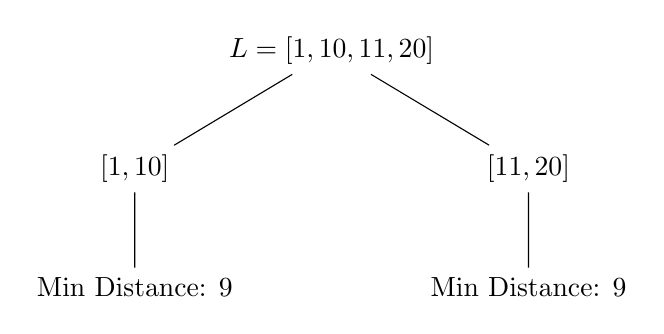
\begin{tikzpicture}
		\tikzstyle{level 1}=[sibling distance=50mm]
		\tikzstyle{level 2}=[sibling distance=10mm]
		\node {$L = [1, 10, 11, 20]$}
		child {node {$[1, 10]$}
			child {node{Min Distance: $9$}}}
		child {node{$[11, 20]$}
			child{node{Min Distance: $9$}}};
	\end{tikzpicture}\\
\end{center}
\end{proof}
\end{required}



%%%%%%%%%%%%%%%%%%%%%%%%%%%%%%%%%%%%%%%%%%%%%%%%%%

\end{document} % NOTHING AFTER THIS LINE IS PART OF THE DOCUMENT
